\documentclass{standalone}
%\documentclass{minimal}
\usepackage{xcolor}
\usepackage{pgfplots}
\usepackage{pgfplotstable}
\pgfplotsset{compat=newest}

\begin{document}

\pgfplotstableread{DataTest2.dat}{\firsttable}
  \pgfplotstablegetrowsof{DataTest2.dat}
  \pgfmathtruncatemacro{\rows}{\pgfplotsretval-1}      
\begin{tikzpicture}

\begin{axis}[view={110}{30},axis equal,
    xmin = 0,
    ymin = 0,
    xmax = 3,
    ymax = 3,
    zmin = -1,
    zmax = 4]
\definecolor{bouteillo}{RGB}{0,0,255}

\pgfmathsetmacro{\cubex}{30}
\pgfmathsetmacro{\cubey}{30}
\pgfmathsetmacro{\cubez}{30}

\pgfdeclareplotmark{realcube}{
\fill [orange] (\cubex/2,\cubey/2,\cubez) -- ++(-\cubex,0,0) -- ++(0,-\cubey,0) -- ++(\cubex,0,0) -- cycle;
\fill [green] (\cubex/2,\cubey/2,\cubez) -- ++(0,0,-\cubez) -- ++(0,-\cubey,0) -- ++(0,0,\cubez) -- cycle;
\fill [bouteillo] (\cubex/2,\cubey/2,\cubez) -- ++(-\cubex,0,0) -- ++(0,0,-\cubez) -- ++(\cubex,0,0) -- cycle;
    }
    
  \pgfmathtruncatemacro{\test}{10}
    
  \colorlet{redhsb}[hsb]{red}%
  \colorlet{bluehsb}[hsb]{blue}%
  %\colorlet{collo}[rgb]{bluehsb!\test!redhsb}
  
\foreach \p in {0,...,\rows}{
		\pgfplotstablegetelem{\p}{[index] 0}\of{\firsttable} 
	  	\let\x\pgfplotsretval 
	  	\pgfplotstablegetelem{\p}{[index] 1}\of{\firsttable} 
	  	\let\y\pgfplotsretval 
	  	\pgfplotstablegetelem{\p}{[index] 2}\of{\firsttable} 
	  	\let\z\pgfplotsretval 
	  	\pgfmathparse{(0 + \z*(0.5/0.125))*100}
	  	 \pgfmathtruncatemacro{\rouge}{\pgfmathresult}
	  	%\definecolor{bobo}{RGB}{\rouge,0,0}	  	
   		%\colorlet{collo}[rgb]{bluehsb!\rouge!redhsb}
   		\edef\temp{
   			%\noexpand\definecolor{bobo}{RGB}{\rouge,0,0}
   			%\noexpand\colorlet{collo}[rgb]{bluehsb!\rouge!redhsb}
   			\noexpand\addplot3 [scatter,mark=realcube,color=red]%
       		%coordinates{(\x,\y,\z)} node [{{RGB}{\rouge,0,0}}, below] {\z};
       		%coordinates{(\x,\y,\z)} node [bobo, below] {\z};
       		coordinates{(\x,\y,\z)} node [color=red, below] {\rouge};
       		%\draw[fill=col,line width=.1pt] (\x*.1,\y*.1) rectangle ++(.1,.1);
   		}
   		%\show\temp %-- uncomment this to see what the \temp macro does
   		\temp
} 
   
\end{axis}

\foreach \iter in {0,...,2}{%
	\node [-latex] at ({\iter},0) {$\iter$}  ;
}

\end{tikzpicture}

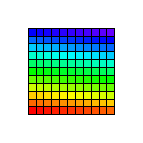
\begin{tikzpicture}
  \colorlet{redhsb}[hsb]{red}%
  \colorlet{bluehsb}[hsb]{blue}%
  \foreach \x in {0,...,10}{
    \foreach \y in {0,...,10}{
      \pgfmathtruncatemacro{\rat}{\y*10+\x}
      \colorlet{col}[rgb]{bluehsb!\rat!redhsb}
      \draw[fill=col,line width=.1pt] (\x*.1,\y*.1) rectangle ++(.1,.1);
    }
  }
\end{tikzpicture}

\end{document}